\documentclass[12pt]{article}
\usepackage[brazilian]{babel}
\usepackage[bottom=2.0cm,top=2.0cm,left=2.0cm,right=2.0cm]{geometry}
%\usepackage{fontspec}
\usepackage{indentfirst}
\usepackage{hyperref}
\usepackage{listings}
\usepackage{graphicx}
\usepackage{tabularray}
\usepackage{float}
\usepackage{amsmath}
\usepackage[alf]{abntex2cite}
\usepackage{quoting}
\usepackage[oldvoltagedirection,siunitx,american]{circuitikz}

%\AddToHook{cmd/section/before}{\clearpage}
\setkeys{Gin}{width=0.75\linewidth}

\linespread{1.25}
\parindent=1.25cm

\renewcommand{\lstlistingname}{Código}
\renewcommand{\lstlistlistingname}{Lista de códigos}
\lstset{
  language=Python,
  frame=single,
  framerule=0pt,
  framextopmargin=3ex,
  framexbottommargin=3ex,
  framexleftmargin=1em,
  xleftmargin={\dimexpr 1em+3pt},
  breaklines=true,
}

\hypersetup{colorlinks,citecolor=black,filecolor=black,linkcolor=black,urlcolor=black}

\title{Projeto de circuitos elétricos usando estratégias evolutivas}
\author{Jaedson Barbosa Serafim}
\date{\today}

\begin{document}

\maketitle

\tableofcontents

\clearpage
\section{Introdução}

Neste trabalho foi feito o cálculo dos valores de resistências para a máxima transferência de energia para o resistor $R_L$ no circuito \ref{fig:circuito} usando estratégias evolutivas.

\begin{figure}
    \centering
    \begin{circuitikz}
        \draw (0,0)
        to[V=$V_{in}$] (0,2)
        to[R=$R_1$] (2,2)
        to[R, l_=$R_2$, *-*] (2,0) -- (0,0)
        (2,2) -- (4,2)
        to[R=$R_L$] (4,0) -- (2,0)
        (3, 2) to [open,v=$V_1$] (3, 0);
    \end{circuitikz}
    \caption{Circuito em análise.}
    \label{fig:circuito}
\end{figure}

A vantagem deste circuito é que, dada a sua simplicidade, é possível facilmente saber qual a resposta para solução do problema. A máxima transferência de energia ocorre quando o resistor $R_1$ é substituído por um curto, que pode ser interpretado como uma resistência muito pequena, enquanto o resistor $R_2$ é substituído por um aberto, interpretável como uma resistência muito grande, obtendo assim o circuito equivalente \ref{fig:circuito-eq}.

\begin{figure}
    \centering
    \begin{circuitikz}
        \draw (0,0)
        to[V=$V_{in}$] (0,2) -- (2,2)
        to[R=$R_L$] (2,0) -- (0,0);
    \end{circuitikz}
    \caption{Circuito de máxima transferência de energia.}
    \label{fig:circuito-eq}
\end{figure}

A potência dissipada pelo resistor $R_L$ no circuito equivalente \ref{fig:circuito-eq} pode ser calculada usando a equação \ref{eq:formula_simplificada}.

\begin{equation}
    \label{eq:formula_simplificada}
    P_{max} = \frac{V_{in}^2}{R_L}
\end{equation}

Substituindo $V_{in}$ por $10V$ e $R_L$ por $50\Omega$ na equação \ref{eq:formula_simplificada} chega-se à máxima potência teórica para  resistência $R_L$ no circuito \ref{fig:circuito}:

\begin{equation}
    \label{eq:potencia_teorica}
    P_{max} = \frac{10^2}{50} = 2W
\end{equation}

Nessa simplificação da figura \ref{fig:circuito-eq}, como não há outros elementos resistivos no circuito, toda a potência fornecida pela fonte é entregue à resistência, ou seja, o rendimento do circuito é de 100\%.

\section{Função de rendimento}
\label{cap:equacionament}

A função da potência de saída do circuito \ref{fig:circuito} pode ser definida como sendo:

\begin{equation}
    \label{eq:pout}
    P_{out} = \frac{V_1^2}{R_L}
\end{equation}

$V_1$ pode ser escrito em função de $V_{in}$ e das resistências:

\begin{equation}
    \label{eq:v1}
    \begin{split}
        V_1 & = V_{in} * \frac{R_2\parallel R_L}{R_1 + R_2\parallel R_L} \\
        & = V_{in} * \frac{1}{1 + \frac{R1}{R_2\parallel R_L}} \\
        & = V_{in} * \frac{1}{1 + \frac{R1}{\frac{R_2 * R_L}{R_2 + R_L} }} \\
        & = V_{in} * \frac{1}{1 + R1 * \frac{R_2 + R_L}{R_2 * R_L} }
    \end{split}
\end{equation}

Por fim, a potência de entrada do circuito \ref{fig:circuito} é definida por:

\begin{equation}
    \label{eq:pin}
    P_{in} = V_{in} * \frac{V_{in} - V_1}{R_1}
\end{equation}

Usando as equações \ref{eq:pout}, \ref{eq:v1} e \ref{eq:pin} é possível então calcular a eficiência do circuito, ou seja, a relação entre a potência de saída e a potência de entrada, dada pela fórmula:

\begin{equation}
    \label{eq:n}
    \eta = \frac{P_{out}}{P_{in}}
\end{equation}

\section{Análise inicial}

Existem resistores com diversos valores de resistência, mas aqui a busca foi limitada de $1m\Omega$ a $100k\Omega$, que é um intervalo de busca bem abrangente caso fosse usada uma escala linear, por isso foi adotada uma escala logarítmica, para reduzir o intervalo de busca para $\left[-2,5\right]$.

\lstinputlisting[label=code:preanalise, caption={Análise inicial do problema.}]{pre_analysis.py}

Usando como base as fórmulas do capítulo \ref{cap:equacionament} foi escrito o código \ref{code:preanalise}, responsável por plotar algumas figuras que nos ajudam a entender melhor o problema.

\begin{figure}
    \centering
    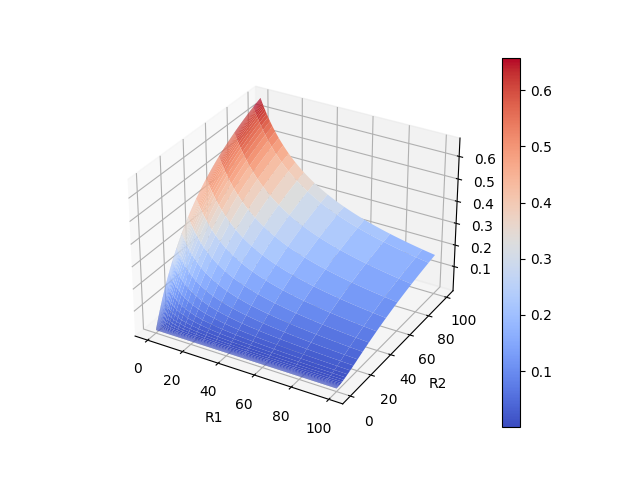
\includegraphics{fig/surface.png}
    \caption{Eficiência em função de $R_1$ e $R_2$.}
    \label{fig:ef}
\end{figure}

A figura \ref{fig:ef} demonstra que não existem máximos locais na função avaliada, apenas um máximo global, o que facilita a sua busca, embora este esteja nos extremos do domínio da busca, o que dificulta sua descoberta, ou seja, é bem difícil chegar ao ponto exato de máximo global, mas é fácil chegar próximo dele.

\begin{figure}
    \centering
    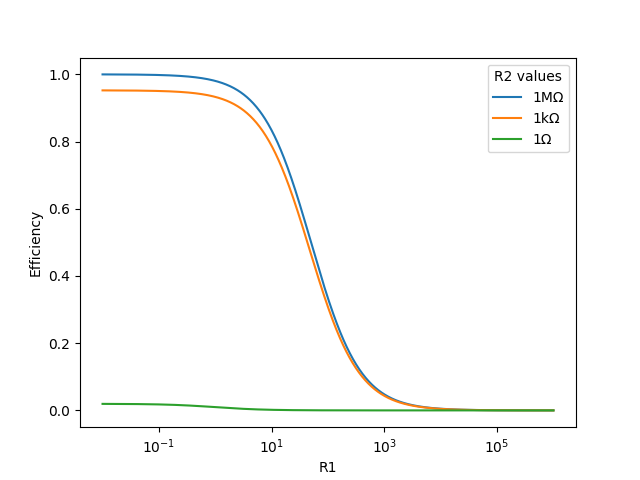
\includegraphics{fig/efficiency_vs_r1.png}
    \caption{Curvas de eficiência em função de $R_1$ para 3 valores distintos de $R_2$.}
    \label{fig:efr1}
\end{figure}

\begin{figure}
    \centering
    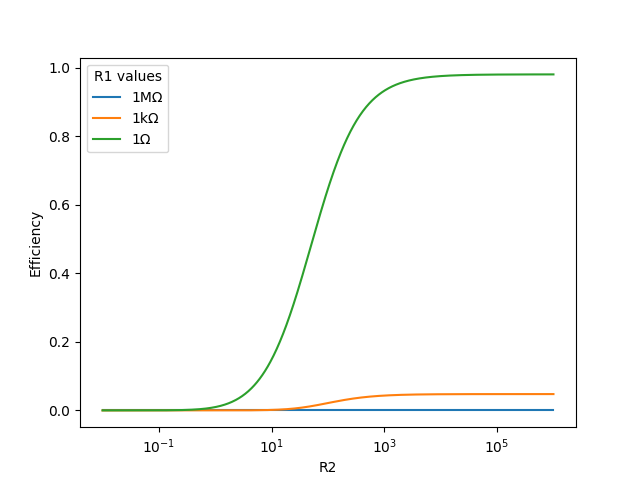
\includegraphics{fig/efficiency_vs_r2.png}
    \caption{Curvas de eficiência em função de $R_2$ para 3 valores distintos de $R_1$.}
    \label{fig:efr2}
\end{figure}

As figuras \ref{fig:efr1} e \ref{fig:efr2} foram plotadas com o eixo \textit{X} em escala logarítmica e assim a curva exibida tornou-se "legível", comprovando que a melhor forma de buscar os melhores valores de $R_1$ e $R_2$ é analisando em potências de 10.

\section{Função de \textit{fitness}}

\lstinputlisting[label=code:simulacao, caption={Simulação do circuito usando PySpice.}]{simulation.py}

Muitas vezes é necessário usar ferramentas externas para a solução de um problema e aqui não é diferente, por isso a biblioteca PySpice é importada na primeira linha do código \ref{code:simulacao}, para simular o circuito e assim obtermos o valor da tensão $V_1$, usada para calcular as potências e assim conseguirmos o rendimento do circuito. "Por baixo dos panos", o que esta biblioteca faz é passar os parâmetros para outro programa, o Ngspice, e interpreta suas respostas.

\section{Estratégias evolutivas}

\lstinputlisting[label=code:ag, caption={Algoritmo genético com codificação binária.}]{index.py}

O algoritmo usado neste trabalho é na verdade um aprimoramento do criado por \citeonline{brownlee_simple_2021}, que embora funcionasse razoavelmente bem, não atendia a todas as solicitações deste projeto.

Esse código tem implementada a forma mais simples de algoritmo genético, sempre priorizando a aleatoriedade do processo e a simplicidade do algoritmo, assim alguns parâmetros são fixos em todos as execuções deste algoritmo a partir da função \textit{main}, são eles:

\begin{itemize}
    \item intervalo de valores (\textit{r\_range}) igual a $\left[-2,5\right]$;
    \item alvo (\textit{target}) igual a $0,99$, ou seja, 99\% da energia fornecida pela fonte é dissipada na resistência $R_L$;
    \item simulação limitada a 50 iterações;
    \item 2 simulações por chamada da função \textit{main}, garantindo resultados mais precisos; e
    \item taxa de mutação dividida pela quantidade de variáveis de cada indivíduo, assim o valor enviado à função é referente à probabilidade de um indivíduo ter uma mutação em alguma de suas características.
\end{itemize}

\begin{quoting}[rightmargin=0cm,leftmargin=4cm]
\begin{singlespace}
{\footnotesize 
O AG básico descarta a geração anterior e considera para a futura apenas os descendentes obtidos. A técnica Elitista consiste em reintroduzir o indivíduo melhor avaliado de uma geração para a seguinte, evitando a perda de informações importantes presentes em indivíduos de alta avaliação e que podem ser perdidas durante os processos de seleção e cruzamento. Algumas técnicas controlam o número de vezes que o indivíduo pode ser reintroduzindo, o que contribui para evitar convergência a máximos locais. \cite[p. 6]{bento_algoritmos_2008}
}
\end{singlespace}
\end{quoting}

Apesar do operador de elitismo muitas vezes contribuir para uma maior velocidade de convergência, ele cria alguns problemas como a maior probabilidade de estagnação em um máximo local, como pôde ser percebido no último trabalho, além de também acrescentar uma nova camada de complexidade à solução e dificultar o seu processamento em paralelo para conjuntos de dados muito extensos. Além de que, uma menor taxa de cruzamento aumenta a probabilidade dos bons indivíduos continuarem dentre a população e a correta escolha desse parâmetro faz com que o algoritmo não seja tão penalizado pela ausência do operador de elitismo. Em outras palavras, a taxa de elitismo é igual a zero em todas as execuções.

\section{Simulações}

\lstinputlisting[label=code:final, caption={Simulações e plotagem de gráficos.}]{sim_and_plots.py}

Resumidamente, o código \ref{code:final} chama a função \textit{main} com 5 diferentes taxas de cruzamento, definidas na variável \textit{r\_cross\_opts}, e 4 diferentes taxas de mutação, armazenadas em \textit{r\_mut\_opts}, e armazena os resultados em 4 diferentes vetores, cada um com um tipo de seleção e um tamanho populacional diferente. Por fim, esses resultados são plotados nos gráficos exibidos no próximo capítulo.

\section{Resultados}

Com apenas 2 minutos de processamento foi possível chegar aos resultados que serão discutidos neste capítulo. Começando com  a figura \ref{fig:fitgeral}, ela mostra o nível extremo de aleatoriedade deste algoritmo e sua incrível capacidade de quase sempre convergir ao ponto correto em poucas iterações. As poucas população que não o fizeram, só não conseguiram por causa do limite imposto de apenas 25 iterações, mas é interessante notar que todas estavam muito próximas de chegar ao resultado final.

\begin{figure}
    \centering
    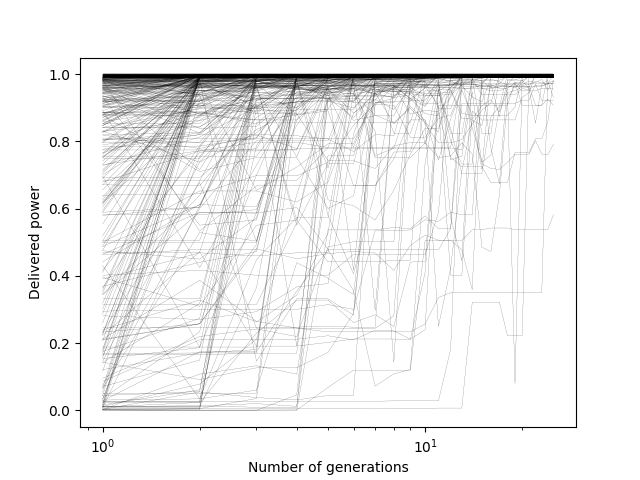
\includegraphics{fig/generations.png}
    \caption{Melhores \textit{fitness} de 400 simulações aleatórias diferentes com diferentes parâmetros.}
    \label{fig:fitgeral}
\end{figure}

A quantidade de simulações é igual ao produtório do número de:

\begin{itemize}
    \item simulações para cada chamada da função \textit{main}: 2;
    \item taxas de mutação: 4, são elas: 50\%, 100\%, 150\%, 200\% por indivíduo ou respectivamente 3,125\%, 6,25\%, 9,375\% e 12,5\% por bit;
    \item taxas de cruzamento: 5, são elas: 60\%, 70\%, 80\%, 90\% e 100\%; e
    \item conjuntos de teste: 4, são eles: população de 4 indivíduos com seleção de roleta, população de 4 indivíduos com seleção de torneio, população de 8 indivíduos com seleção de roleta e população de 8 indivíduos com seleção de torneio.
\end{itemize}

Daí vem a quantidade de 160 simulações, das quais 158 convergiram, ou seja, é uma taxa de sucesso de 98,75\%, mesmo com a limitação de apenas 50 gerações.

\begin{figure}
    \centering
    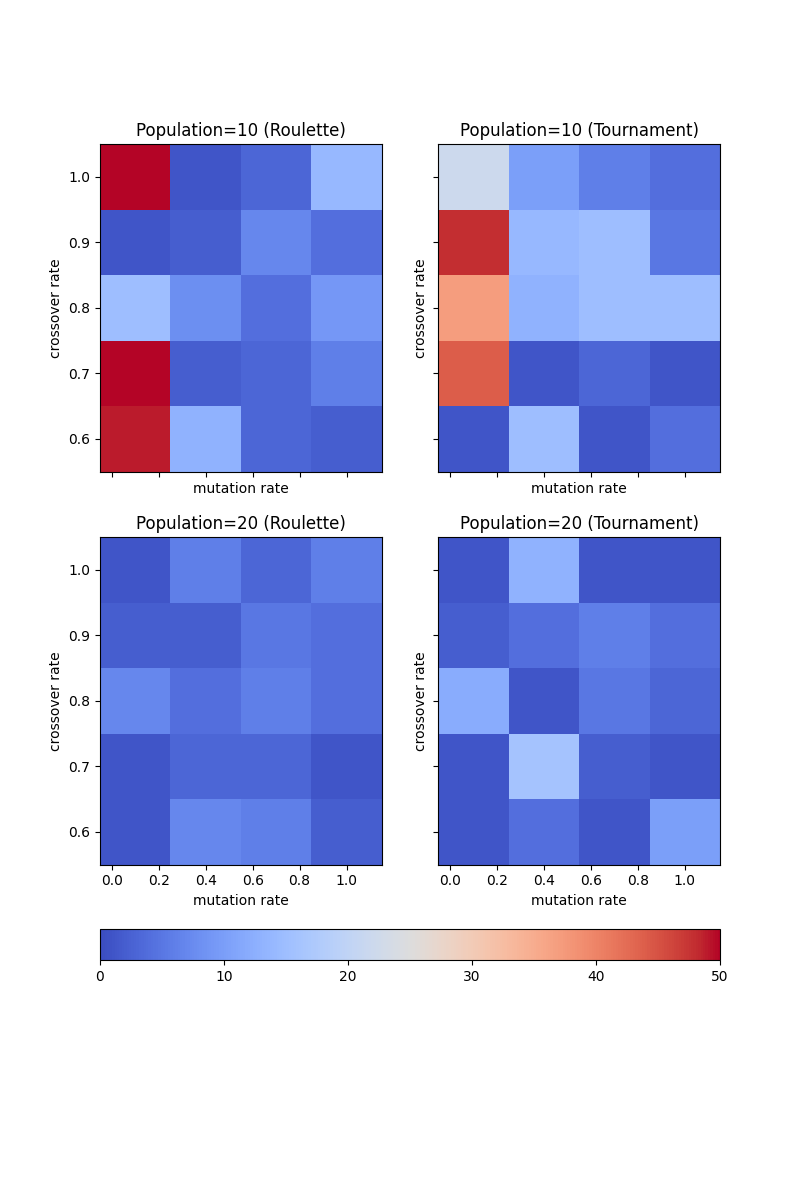
\includegraphics{fig/max_colors.png}
    \caption{Quantidade máxima de gerações para convergir em cada uma dos 4 diferentes conjuntos de teste.}
    \label{fig:max}
\end{figure}

\begin{figure}
    \centering
    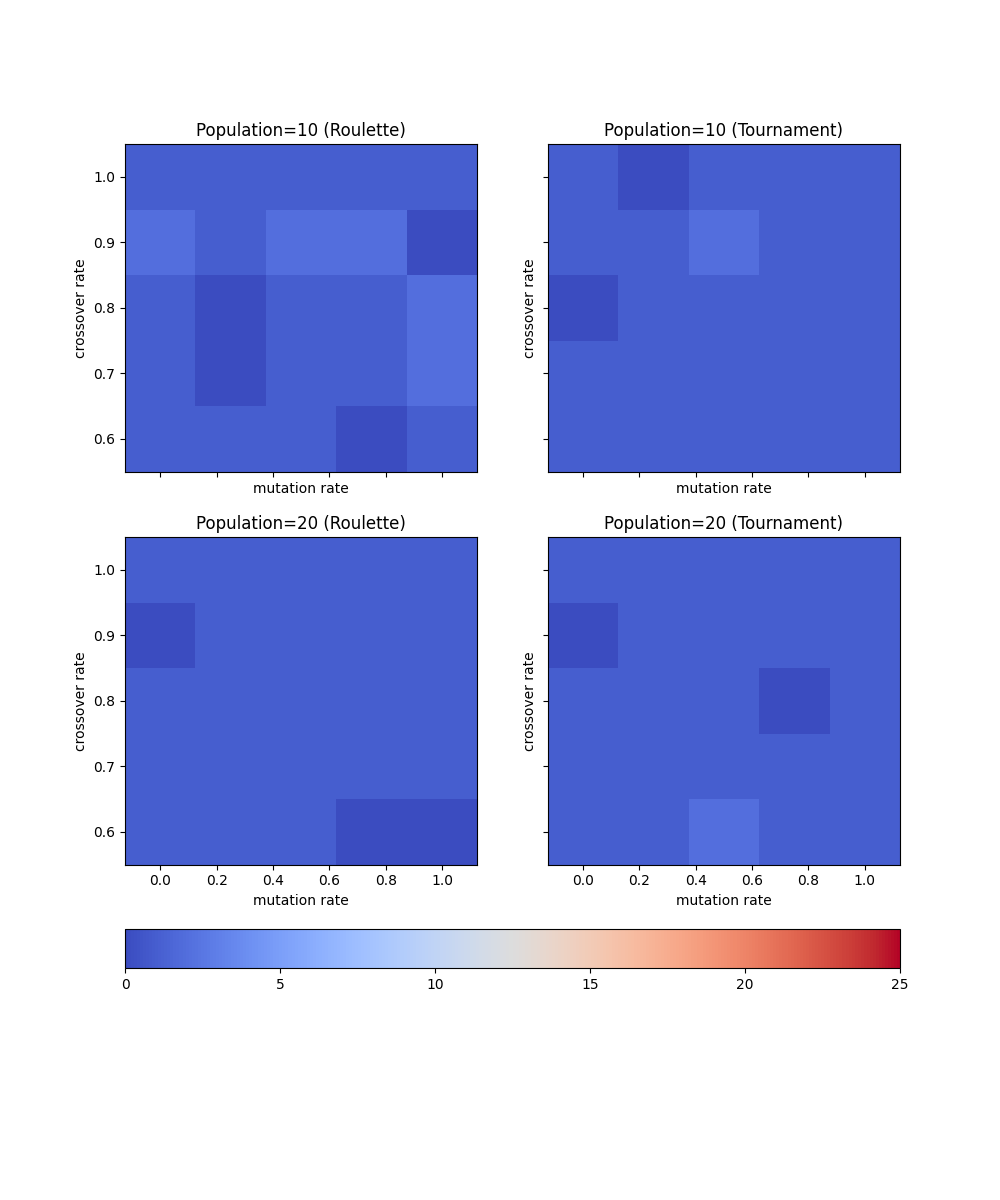
\includegraphics{fig/min_colors.png}
    \caption{Quantidade mínima de gerações para convergir em cada uma dos 4 diferentes conjuntos de teste.}
    \label{fig:min}
\end{figure}

Na figura \ref{fig:min} é possível tirar a conclusão de que com qualquer um dos parâmetros adotados é possível chegar a um resultado satisfatório dependendo da sorte de ter uma boa população inicial.

Na figura \ref{fig:max} é possível visualizarmos o pior resultado das 2 simulações para diferentes tamanhos de população, taxas de cruzamento e mutação com cada um dos métodos de seleção. Ela confirma o que a figura \ref{fig:fitgeral} já dava indícios: no geral foram necessários menos de 5 iterações para se chegar ao resultado esperado, ou seja, quase sempre com poucas simulações foi possível chegar a um resultado que necessitaria milhares de simulações caso todos os valores possíveis fossem ser analisados por meio da força bruta.

\section{Conclusão}

Embora o problema a ser resolvido tenha sido relativamente simples, com ele foi possível aprender um pouco mais sobre como esse tipo de algoritmo pode ser usado para resolver problemas de engenharia de forma eficiente.

\clearpage
\bibliography{citations}

\end{document}